\documentclass[../main/main.tex]{subfiles}

% Put everything that shall appear in the method
% inside this document environment.
\begin{document}
	
	\textbf{Task: describe your ideas and your realization of the task}
	
	\subsection{Designing the Questionnaire}
	
	We started out by designing a questionnaire in \LaTeX and using the corporate design of our university. We separated each task clearly from the one another and wrote the instructions in the headline. The body of each tasks consists of task related information on the left, space for the answer in the middle and an empty coordinate system on the right. It was important to us to keep this structure to increase reliability across the tasks.
	
	We decided to use sorting tasks, because of their high objectivity (see section \ref{sec:discussion} for a discussion on question types). The first seven tasks were closed-form sorting tasks. Directly after executing each task, the subjects were asked to fill out the coordinate system with a probability density function over their performance. We decided to ask the subjects to sort five terms in a predefined order. We decided to use two easy items, three medium and two hard items. We randomized the location of the items as well as the order of the answer possibilities. An example can be seen in figure \ref{fig:example-task}.
	
	\begin{figure}[h]
		\label{fig:example-task}
		\centering
		\captionsetup{justification=centering}
		\fbox{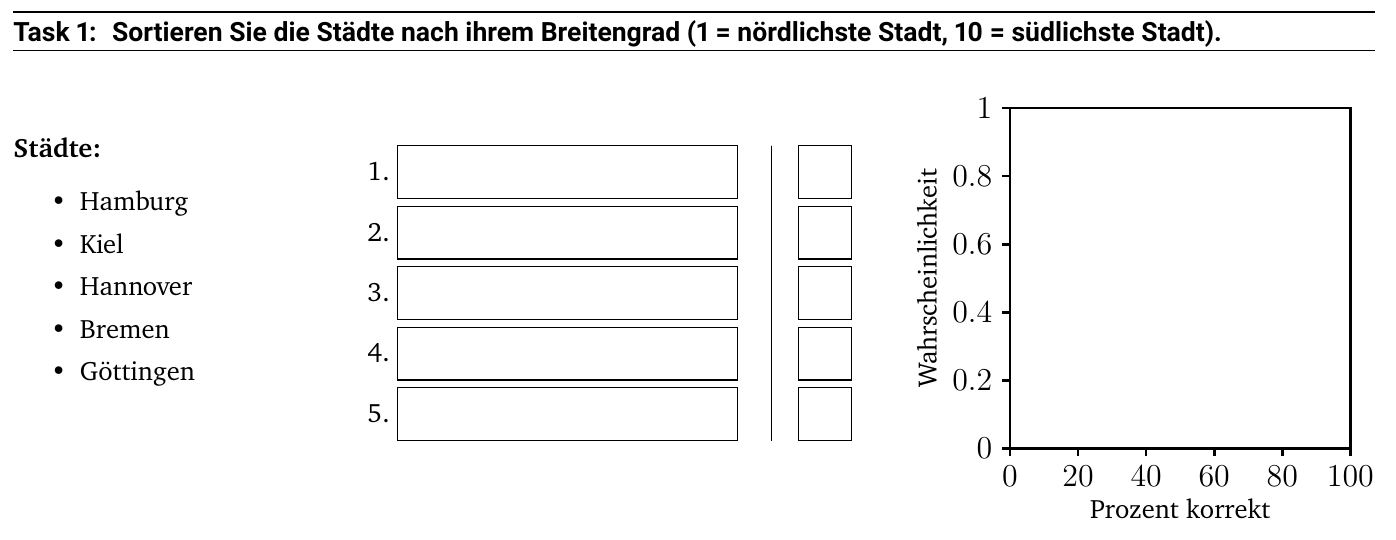
\includegraphics[width=.8\textwidth]{../assets/example-task-1.png}}
		\caption{Example closed-form sorting task.}
	\end{figure} 
	
	After the seven tasks, we asked the subjects to estimate their performance over all the previous tasks, by drawing another probability density function. With this we want to learn how well humans can average their performance on several task. 
		
	 The eighth task was an open end sorting tasks, which we decided to incorporate out of curiosity how the self-assessment would change in comparison to closed form sorting tasks. The task can be seen in figure \ref{fig:example-task2}.
	 
	 \begin{figure}[h]
	 	\label{fig:example-task2}
	 	\centering
	 	\captionsetup{justification=centering}
	 	\fbox{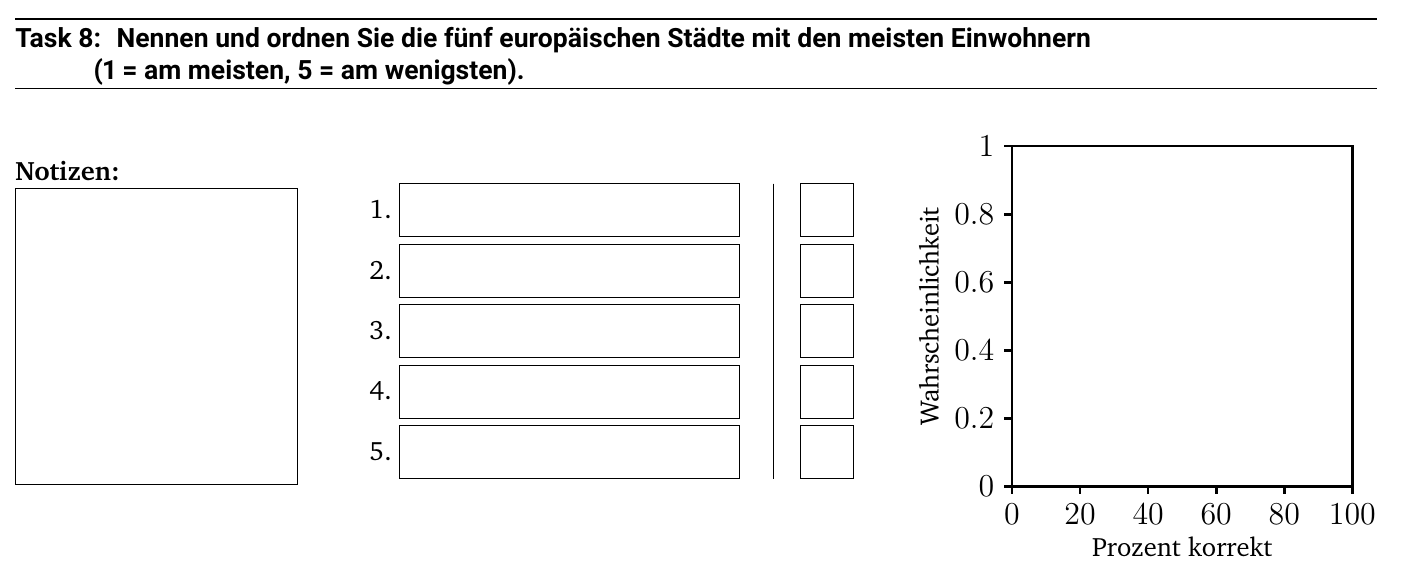
\includegraphics[width=.8\textwidth]{../assets/example-task-8.png}}
	 	\caption{Example open end sorting task.}
 	\end{figure} 
	 

	\subsection{Processing Pipeline}
	
	\subsection{Extracting Probability Density Functions}
	
	To extract the probability density functions from a scanned PDF into an image, we used computer vision to detect the probability density functions on the JPEG and simply cut out the detected regions from the JPEG. The cutout process is fairly easy. In python, images are stored as an array of numbers. As soon as we get the area of the pdf as pixels, we can simply enter these pixel indices in the array and extract that part of the image. Then we save it using OpenCV a free computer vision library in python.
	
	The hard part is to identify the probability density functions in the image. However, we designed our questionnaire in a way that reduces the detection of the pdf to the detection of a big square. If we can reliably detect the coordinate system, which the subjects use to draw their pdfs in, we can extract the pdf if we only look at the pixels which lie inside this square.
	
	To detect squares, we need to detect vertical and horizontal lines first. We did exactly that and looked at all contours that could be build with horizontal and vertical lines. This will output all lines on their own, but also all triangles, rectangles and squares. Everything that forms a contour. Now we sorted the contours. It is important to sort the contours (or later pdfs), regarding their position on the page. To the computer all pdfs look the same, so we have to make sure that we assign the correct pdf to the correct task. Because all tasks are ordered in ascending order, we can sort the pdfs from north to south.
	
	Next, we had to find the correct square from the contours. We did this by iterating over the contours and testing each contour on some

\end{document}